\scanpage{6}
\mspage{4}
\margin{\figure{\begin{tikzpicture}\draw (0,0) .. controls (.2,-.3) and (.5,-.45) .. (.6,-.7);\end{tikzpicture}}}

\figure{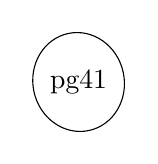
\begin{tikzpicture}[baseline=(t.base)]\node[inner sep=3pt] (t) {\uline{pg41}};\draw[rotate=12] (0,0) ellipse (0.58 and 0.63);\end{tikzpicture}}
$\ell-2$\quad ``fonction de Dirac'' est malheureux (sur un groupe, on ne \unsure{voit|sait} trop si c'est\quad ou
\diagram{\left\{\begin{array}{l} f(e)=1,\ 0\ \text{ailleurs}\\ f(e)=\#G,\ 0\ \text{ailleurs}\end{array}\right.})
\margin{\unsure{guillemets suffisent} ?}

\uline{pg42}\quad début dém. 4.7 : le \unsure{eps|cas} n'est pas clair pour $n=2$, et je n'ai pas confiance en dehors du cas strictement local.

\figure{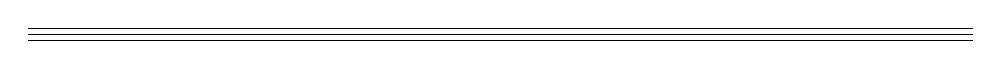
\begin{tikzpicture}\draw (0,0)--(12,0);\draw (0,-0.08)--(12,-0.08);\draw (0,-0.16)--(12,-0.16);\end{tikzpicture}}

\figure{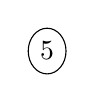
\begin{tikzpicture}[baseline=(t.base)]\node (t) {5};\draw (0,0) ellipse (0.24 and 0.29);\end{tikzpicture}}

\uline{pg\unsure{45|47}}\quad $\ell\,3$ ss\quad français : beaucoup de ``donc''.

\uline{pg46}\quad Quel est le sens de (5.2.3.1) et de \deleted{\unsure{le}} ``par définition'' qui suit --

S'agit-il de pro-objets, ou de schémas.
\margin{\figure{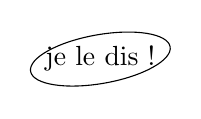
\begin{tikzpicture}[baseline=(t.base)]\node (t) {je le dis !};\draw[rotate=10] (0,0) ellipse (0.90 and 0.31);\end{tikzpicture}}}

\uline{pg48}\quad $\ell-4$\quad Pourquoi as-tu barré connexe ?

\deleted{\uline{pg53}\quad 5.7 est une redite pour $\ell\ne p$, et un peu idiot pour $\ell=p$.}\quad (utilisé en 5.15)

\figure{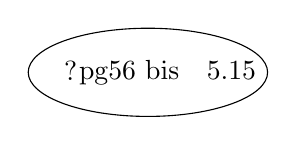
\begin{tikzpicture}[baseline=(t.base)]\node[inner sep=3pt] (t) {\uline{pg56 bis}\quad 5.15};\node at (-1.23,0.02) {?};\draw (-0.25,0) ellipse (1.52 and 0.56);\end{tikzpicture}}
tu n'a plus besoin ici de $\operatorname{car}(k)\ne\ell$

54 quater -- 5.11.\quad seraient plutôt que seront.

\uline{55 ter}\quad $\ell-10$. Il serait honnête de dire que 6.6 utilise $\operatorname{car}(K)=0$, via Tate
\margin{\figure{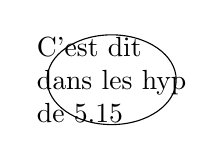
\begin{tikzpicture}[baseline=(t.base)]\node[align=left] (t) {C'est dit\\dans les \unsure{hyp}\\de 5.15};\draw (0,0) ellipse (0.82 and 0.57);\end{tikzpicture}}}

\figure{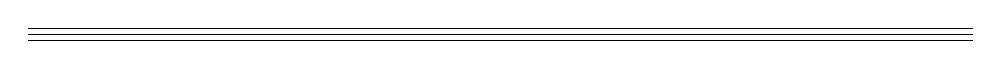
\begin{tikzpicture}\draw (0,0)--(12,0);\draw (0,-0.08)--(12,-0.08);\draw (0,-0.16)--(12,-0.16);\end{tikzpicture}}

\figure{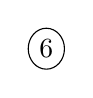
\begin{tikzpicture}[baseline=(t.base)]\node (t) {6};\draw (0,0) ellipse (0.23 and 0.26);\end{tikzpicture}}

\uline{pg57/58} : tu supposes tantôt $A^0$ $\ell$-divisible $(58,\ell-11)$, tantôt non $(57,\ell\,3)$

\uline{pg58}\quad $\ell-5$\quad
\figure{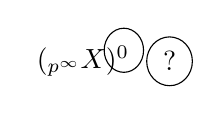
\begin{tikzpicture}[baseline=(t.base)]\node (t) {$( {}_{p^\infty}X)^0$};\draw (0.52,0.14) ellipse (0.25 and 0.28);\node at (1.10,0) {?};\draw (1.10,0) ellipse (0.29 and 0.31);\end{tikzpicture}}
\qquad itou plus loin --

\uline{pg59}\quad Je ne comprends rien -- Que fais-tu de la partie discrète ? --
\margin{\uline{CANULAR ?!}}

Je ne crois pas que la plus grande \deleted{\unsure{VA}} sous VA ordinaire puisse se relever (\unsure{$\hat{\mathrm m}$|ni} en cas de bonne réduction).

\uline{ie}\quad \unsure{6.3|63} est faux (déformer de façon générale $E\times F$, $E$ et $F$ elliptiques, $E$ ordinaire, $F$ non ordinaire ; général $\Rightarrow$ générique simple.

\margin{5}
